\documentclass{article}

\usepackage{graphicx}
\usepackage{tikz}
\usepackage{tikzsymbols}
\usetikzlibrary{calc,patterns,shapes.geometric}
\pagestyle{empty}
\usepackage[margin=0pt]{geometry}
\geometry{papersize={14in,12in}}

\def\centerarc[#1](#2)(#3:#4:#5){\draw[#1] ($(#2)+({#5*cos(#3)},{#5*sin(#3)})$) arc (#3:#4:#5);}

\begin{document}
	\begin{figure}
		\centering
		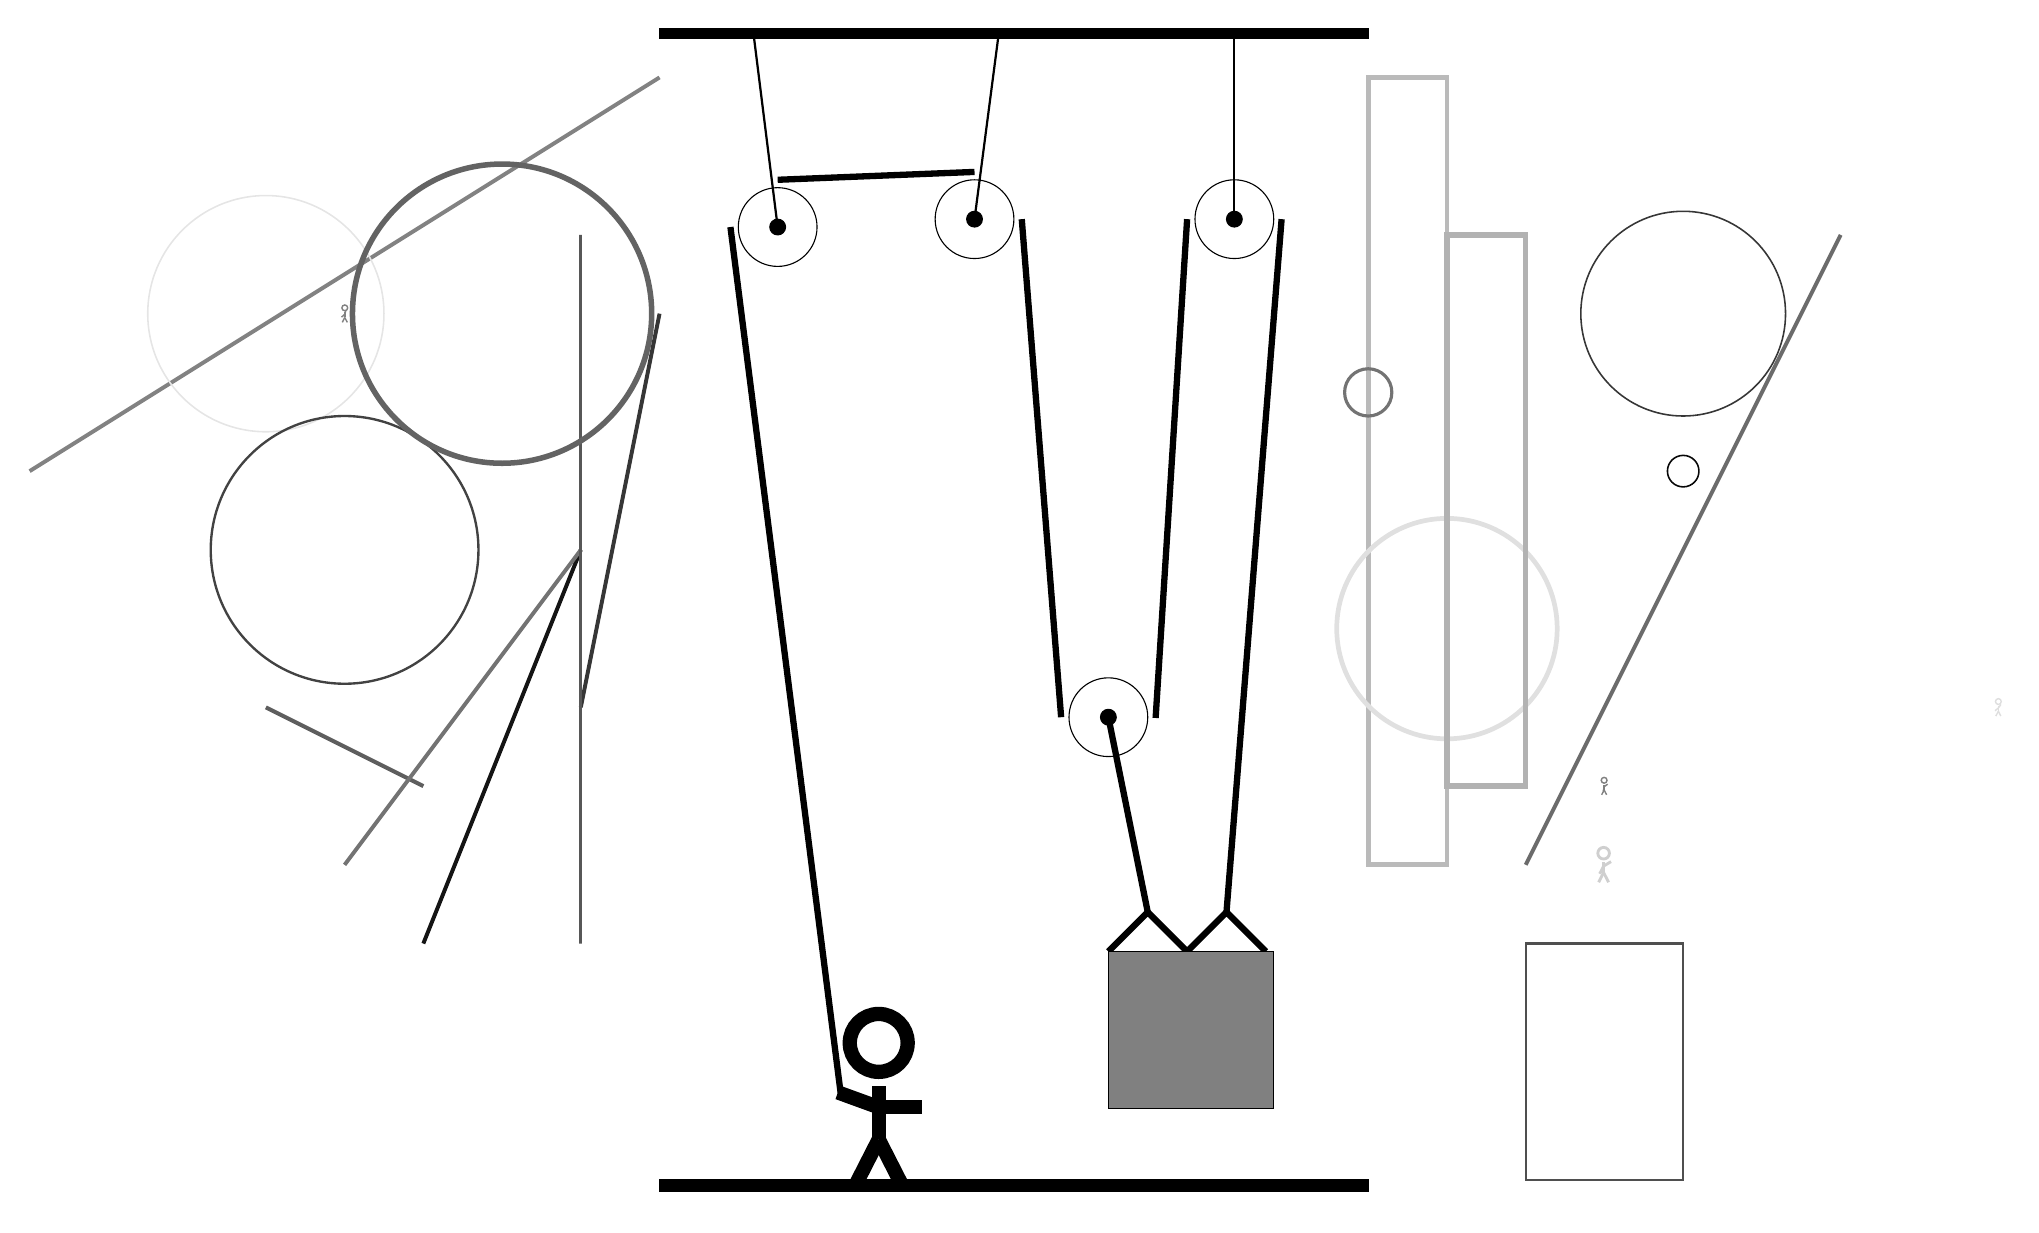
\begin{tikzpicture}
			%%%%% START %%%%%
			
			\draw[fill=black] (-3, 11.5) rectangle (6, 11.625);
			
			\node[line width=0.7mm, color=black!50] at (9, 2) {\Strichmaxerl[1][79][36]};
			
			\draw [line width=0.2mm, color=black!79](10, 8) circle (1.3);
			\draw[line width=0.5mm, color=black!63](-6, 2) -- (-8, 3);
			\draw[line width=0.5mm, color=black!58](8, 1) -- (12, 9);
			
			\node[line width=0.6mm, color=black!19] at (9, 1) {\Strichmaxerl[2][63][31]};
			\node[line width=0.5mm, color=black!49] at (-7, 8) {\Strichmaxerl[1][41][75]};
			\draw[line width=0.3mm, color=black!69] (8, 0) rectangle (10, -3);
			\draw[line width=0.5mm, color=black!49](-3, 11) -- (-11, 6);
			\draw[line width=0.6mm, color=black!27] (7, 1) rectangle (6, 11);
			\draw[line width=0.5mm, color=black!79](-4, 3) -- (-3, 8);
			\draw [line width=0.2mm, color=black!10](-8, 8) circle (1.5);
			\draw [line width=0.3mm, color=black!74](-7, 5) circle (1.7);
			\draw[line width=0.5mm, color=black!92](-4, 5) -- (-6, 0);
			
			\node[line width=0.6mm, color=black!13] at (14, 3) {\Strichmaxerl[1][40][54]};
			\draw [line width=0.6mm, color=black!12](7, 4) circle (1.4);
			\draw[line width=0.5mm, color=black!55](-7, 1) -- (-4, 5);
			
			\draw[line width=0.4mm, color=black!66] (-4, 9) rectangle (-4, 0);
			\draw [line width=0.4mm, color=black!55](6, 7) circle (0.3);
			\draw [line width=0.2mm, color=black!97](10, 6) circle (0.2);
			\draw[line width=0.7mm, color=black!30] (8, 2) rectangle (7, 9);
			\draw [line width=0.7mm, color=black!61](-5, 8) circle (1.9);
			
			\draw (1, 9.2) circle (0.5);
			\draw[fill=black] (1, 9.2) circle (0.1);
			\draw[thick] (1, 9.2) -- (1.3, 11.5);
			
			\draw (4.3, 9.2) circle (0.5);
			\draw[fill=black] (4.3, 9.2) circle (0.1);
			\draw[thick] (4.3, 9.2) -- (4.3, 11.5);
			
			\draw (2.7, 2.875) circle (0.5);
			\draw[fill=black] (2.7, 2.875) circle (0.1);
			
			\draw[line width=0.8mm]  (2.7, -0.1) -- (3.2, 0.4) -- (3.7, -0.1) -- (4.2, 0.4) -- (4.7, -0.1);
			\draw[fill=black!50] (2.7, -0.1) rectangle (4.8, -2.1);
			
			\draw (-1.5, 9.1) circle (0.5);
			\draw[fill=black] (-1.5, 9.1) circle (0.1);
			\draw[thick] (-1.5, 9.1) -- (-1.8, 11.5);
			
			\draw[line width=0.8mm](-0.7, -1.9) --  (-2.1, 9.1);
			\centerarc[line width=0.8mm](-1.5, 9.1)(90:180:0.6);
			\draw[line width=0.8mm](-1.5, 9.7) -- (1, 9.8);
			\centerarc[line width=0.8mm](1, 9.2)(0:90:0.6);
			\draw[line width=0.8mm](1.6, 9.2) -- (2.1, 2.875);
			\centerarc[line width=0.8mm](2.7, 2.875)(180:370:0.6);
			\draw[line width=0.8mm] (3.3, 2.865) -- (3.7, 9.2);
			\centerarc[line width=0.8mm](4.3, 9.2)(0:180:0.6);
			\draw[line width=0.8mm](4.2, 0.4) -- (4.9, 9.2);
			\draw[line width=0.8mm] (3.2, 0.4) -- (2.7, 2.875);
			
			\node at (-0.2, -2) {\Strichmaxerl[10][-20][0]};
			
			\draw[fill=black] (-3, -3) rectangle (6, -3.15);
			
			%%%%% END %%%%%
		\end{tikzpicture}
	\end{figure}	
\end{document}